\section{Data and study context}
\label{sec:data}

\paragraph{Scope.} The study area is Albania, represented as a single node with an aggregate interconnector to
its neighbours (Fig.~\ref{fig:context}). All series are indexed in UTC. Local time (Europe/Tirane) is used only to
shape behavioural demand and price patterns. Monetary values are in 2024 euros, converted from USD at
0.92~EUR/USD. Energies are in MWh, powers in MW and water volumes in hm$^3$.

\begin{figure}[htbp]
\centering
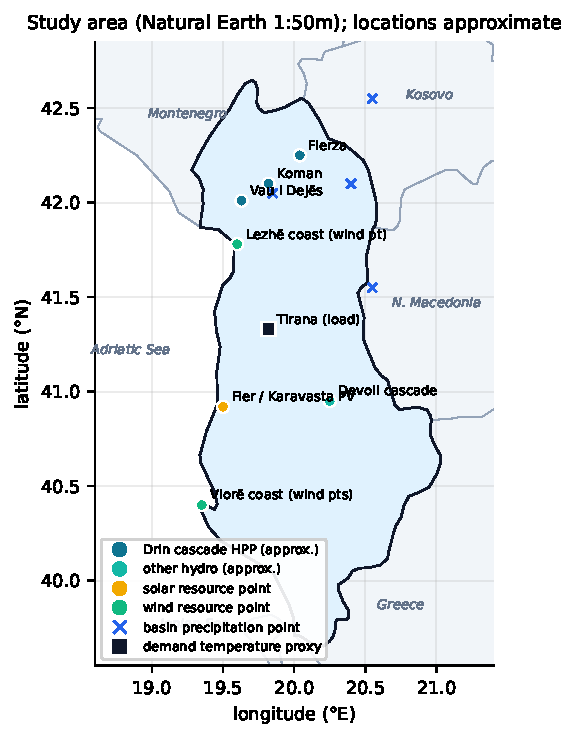
\includegraphics[width=0.48\textwidth]{fig02_study_context.pdf}
\caption{Study area. The Albanian boundary and its neighbours are from Natural Earth 1:50m \cite{naturalearth2026}. Plant
locations are approximate and shown only for orientation; the model itself has no spatial resolution. Crosses
are the four NASA POWER points used to compute basin-mean precipitation for the Drin inflow
reconstruction. Coloured circles are the PV and wind resource points.}
\label{fig:context}
\end{figure}

\paragraph{Meteorological inputs (observed-derived).} Hourly all-sky irradiance, 2-m temperature and 50-m wind
speed for 2019--2023 were retrieved from the NASA POWER point API \cite{nasapower2026} for five points: two
solar (Fier/Myzeqe, Vlorë), two coastal wind (Vlorë--Karaburun, Lezhë--Shëngjin) and a Tirana demand
proxy. Daily bias-corrected precipitation and temperature for 2000--2023 were retrieved for four points in the
Drin basin (White Drin, Black Drin, Kukës/Fierza, Koman). Open-Meteo ERA5 data for Tirana in 2021
\cite{openmeteo2026} were retrieved as a cross-check only. Every dataset has a machine-readable provenance
record (Table~\ref{tab:data-dictionary} in the Appendix).

\paragraph{PV and wind capacity factors (weather-derived).} PV output follows a simplified PVWatts-type model
\cite{dobos2014pvwatts}: horizontal irradiance with a constant tilt gain of 1.10, system losses of 0.86 and a
temperature derating of $-0.4\%/^\circ$C, with cell temperature estimated from a nominal operating cell
temperature (NOCT) of $45^\circ$C. Wind output scales the 50-m wind speed to a 100-m hub height using a shear
exponent of 0.14 and applies a generic 3/12/25~m/s power curve with 0.85 losses. The mean annual capacity
factors are 0.170--0.176 for PV and 0.108--0.119 for wind across 2019--2023. The wind values are low, and are
likely conservative because coarse reanalysis smooths coastal and orographic winds \cite{staffell2016wind}.
These are modelled availabilities, \emph{not measured production}.

\paragraph{Hydrology (reconstructed).} Basin-mean precipitation and temperature drive a degree-day snow model
\cite{hock2003melt} (threshold $0.5^\circ$C, 3~mm/$^\circ$C/day). Its output feeds two parallel linear
reservoirs \cite{beven2012rainfall} with recession constants of 4 and 45 days. The resulting runoff index is
scaled so that the 2001--2023 mean inflow volume yields an \emph{assumed} long-run Drin-cascade energy of
4.1~TWh/yr. This is consistent in magnitude with the reported mean output of about 1.33~TWh for Fierza alone,
the uppermost of the three stages. Run-of-river availability for the remaining hydro fleet (about 930~MW,
Table~\ref{tab:assumptions}) is a normalised blend of fast and total runoff, capped at capacity and scaled to
2.6~TWh/yr. No gauge or plant records were accessible, so the hydrological parameters are uncalibrated
assumptions. The reconstructed annual inflow index (Fig.~\ref{fig:profiles}d) has a 5th percentile of 0.78, a
median of 0.99 and a minimum of 0.67 (2011). The reference weather year, 2022, was selected algorithmically as
the 2019--2023 year closest to the median. This ranking should not be read as the observed hydrology of 2022.

\paragraph{Demand and prices (synthetic).} ENTSO-E Transparency data require a registered token, which was not
used. Hourly demand is therefore \textbf{synthetic}. It is generated from Tirana temperature with assumed
heating (3.0\%/$^\circ$C below $16^\circ$C) and cooling (3.5\%/$^\circ$C above $24^\circ$C) sensitivities, an
assumed diurnal and weekly shape, and AR(1) noise with a fixed seed, and it is scaled to an assumed
8.0~TWh/yr. Its peak is about 1.64~GW. Import prices are also synthetic: the mean is 105~EUR/MWh, with diurnal
and seasonal shapes and multiplicative AR(1) noise. Export revenue is 85\% of the import price, which
represents transmission charges and market spreads. All outputs carry the label \emph{``synthetic research
demonstration data --- not observed grid operations''}.

\begin{figure}[htbp]
\centering
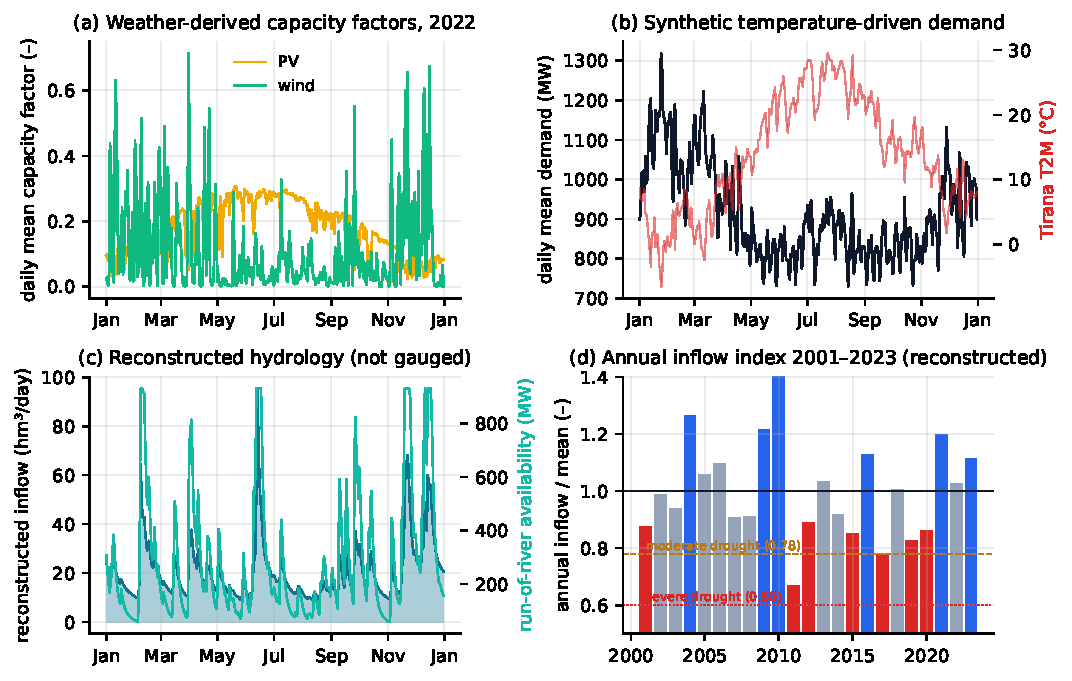
\includegraphics[width=\textwidth]{fig03_profiles.pdf}
\caption{Model inputs for the reference year. (a)~Daily mean PV and wind capacity factors derived from NASA POWER.
(b)~Synthetic temperature-driven demand. (c)~Reconstructed Drin inflow and run-of-river availability.
(d)~Reconstructed annual inflow index for 2001--2023 relative to its mean, with the moderate (0.78) and severe
(0.60) drought scenario levels marked.}
\label{fig:profiles}
\end{figure}

\paragraph{System and cost parameters.} Table~\ref{tab:assumptions} lists all key parameters and their status.
Sourced values are the Drin cascade capacities \cite{kesh2026drin}, the hydro fleet size \cite{irena2021rra} and
the IRENA 2024 technology costs \cite{irena2025costs}. We apply an assumed regional cost multiplier of 1.25
because global weighted averages are dominated by low-cost markets. The remaining values are assumptions
chosen to be of plausible magnitude, and the important ones are varied in Section~\ref{sec:sensitivity}.

\begin{table}[htbp]
\centering
\footnotesize
\caption{Key system and cost parameters. ``Assumption'' marks values chosen for this study that were not taken from an observed Albanian dataset.}
\label{tab:assumptions}
\begin{tabular}{p{5.2cm}lrp{5.0cm}}
\toprule
Parameter & Unit & Value & Source / status \\
\midrule
Drin cascade turbine capacity & MW & 1\,350 & KESH (Fierza 500, Koman 600, Vau i Dejës 250) \\
Aggregate head / efficiency & m / -- & 230 / 0.88 & assumption \\
Energy equivalent $\kappa$ & MWh/hm$^3$ & 551.5 & derived \\
Reservoir $V^{\min}$ / $V^{\max}$ & hm$^3$ & 600 / 2400 & assumption \\
Initial volume (live fraction) & -- & 0.60 & assumption \\
Minimum release & m$^3$/s & 20 & assumption \\
Other hydro (run-of-river aggregate) & MW & 930 & IRENA RRA (2,096 MW, 2018) + Moglicë 184 MW $-$ Drin \\
Existing PV / wind & MW & 300 / 0 & assumption (order of magnitude) \\
Import / export NTC & MW & 900 / 900 & assumption \\
Export price ratio $\rho$ & -- & 0.85 & assumption \\
VOLL & EUR/MWh & 5\,000 & assumption (varied 2,000--10,000) \\
Battery $\eta^c$, $\eta^d$ / min SOC & -- & 0.95, 0.95 / 0.05 & assumption \\
Battery degradation proxy & EUR/MWh & 5.0 & assumption \\
PV capex (incl. ×1.25 regional) & EUR/kW & 795 & IRENA RPGC 2024: USD 691/kW \\
Onshore wind capex (incl. ×1.25) & EUR/kW & 1\,197 & IRENA RPGC 2024: USD 1,041/kW \\
Battery energy capex (incl. ×1.25) & EUR/kWh & 221 & IRENA RPGC 2024: USD 192/kWh \\
Battery power capex (incl. ×1.25) & EUR/kW & 75 & assumption \\
Discount rate / lifetimes & -- / yr & 0.07 / 25, 25, 15 & assumption \\
Annualised PV / wind & kEUR/MW-yr & 80.1 / 132.7 & derived (CRF + FOM) \\
Annualised battery power / energy & kEUR/(MW, MWh)-yr & 10.1 / 29.8 & derived \\
\bottomrule
\end{tabular}
\end{table}


\paragraph{Scenarios.} Each scenario applies a transparent transformation to the reference-year profiles.
Inflows are scaled by $(1-d)$, demand by $(1+g)$ and import prices by $m$, and interconnector availability
is set to $a$ (Table~\ref{tab:scenarios}). The \emph{moderate drought} ($d=0.22$) corresponds to the 5th
percentile of the reconstructed inflow index. The \emph{severe drought} ($d=0.40$) lies beyond the
reconstructed minimum and represents a climate-stress extrapolation. The \emph{compound shock} adds 8\% demand
growth, a 1.8$\times$ import-price shock and a 30\% derating of transfer capacity, all assumed. For two-stage
planning, five scenarios are used. Three come from binning the 23 reconstructed years (wet $>1.10$, normal
0.90--1.10, dry $<0.90$), with their empirical frequencies scaled to 85\% of the probability mass. The other
two are the severe and compound stresses, with an assumed 10\% and 5\%. These probabilities are partly assumed
and are reported as such.

\begin{table}[htbp]
\centering
\small
\caption{Climate and market scenarios. Upper block: named stress presets; lower block: five-scenario set for two-stage planning (historical-bin probabilities from the reconstructed 2001--2023 inflow index, plus an assumed 15\% climate-stress allowance).}
\label{tab:scenarios}
\begin{tabular}{lrrrrr}
\toprule
Scenario & Inflow factor & Demand factor & Import price & NTC avail. & Prob. \\
\midrule
Normal & 1.00 & 1.00 & 1.00 & 1.00 & -- \\
Moderate drought & 0.78 & 1.00 & 1.00 & 1.00 & -- \\
Severe drought & 0.60 & 1.00 & 1.00 & 1.00 & -- \\
Compound shock & 0.60 & 1.08 & 1.80 & 0.70 & -- \\
Wet year (stoch.) & 1.226 & 1.00 & 1.00 & 1.00 & 0.222 \\
Normal (stoch.) & 0.989 & 1.00 & 1.00 & 1.00 & 0.370 \\
Dry year (stoch.) & 0.823 & 1.00 & 1.00 & 1.00 & 0.259 \\
Severe drought (stoch.) & 0.600 & 1.00 & 1.00 & 1.00 & 0.100 \\
Compound shock (stoch.) & 0.600 & 1.08 & 1.80 & 0.70 & 0.050 \\
\bottomrule
\end{tabular}
\end{table}

